\chapter{Conception de la nouvelle solution}

\section{Principe directeur : alerter sur les conséquences plutôt que sur les causes}

La conception proposée repose sur un principe simple mais structurant : une alerte doit représenter
un risque opérationnel clair, compréhensible et actionnable. La personne d'astreinte alertée doit
immédiatement savoir quel service pose problème et quel est l'impact pour l'utilisateur, sans avoir à
corréler manuellement une dizaine de \lexique{métriques} techniques. Pour atteindre cet objectif, quatre règles
de conception ont été retenues :

\begin{itemize}
	\item privilégier les signaux liés aux conséquences d'une panne plutôt qu'à ses seules causes techniques ;
	\item expliciter le niveau de criticité de chaque alerte ;
	\item associer chaque alerte à un périmètre de responsabilité identifié ;
	\item ajouter plus de contexte dans les notifications, afin de faciliter le diagnostic initial et d'accélérer la résolution.
\end{itemize}

\section{Deux points de vue complémentaires : les méthodes RED et USE}

Pour structurer la surveillance, j'ai retenu deux méthodes reconnues de l'ingénierie \lexique{SRE}, en les appliquant à des types de \lexique{métriques} distincts. 
La méthode \lexique{USE} s'applique aux \lexique{métriques} d'infrastructure et adopte une vue « côté machine », tandis que la méthode \lexique{RED} s'applique aux \lexique{métriques} d'application et adopte une vue « côté client ».

\begin{figure}[h]
	\centering
	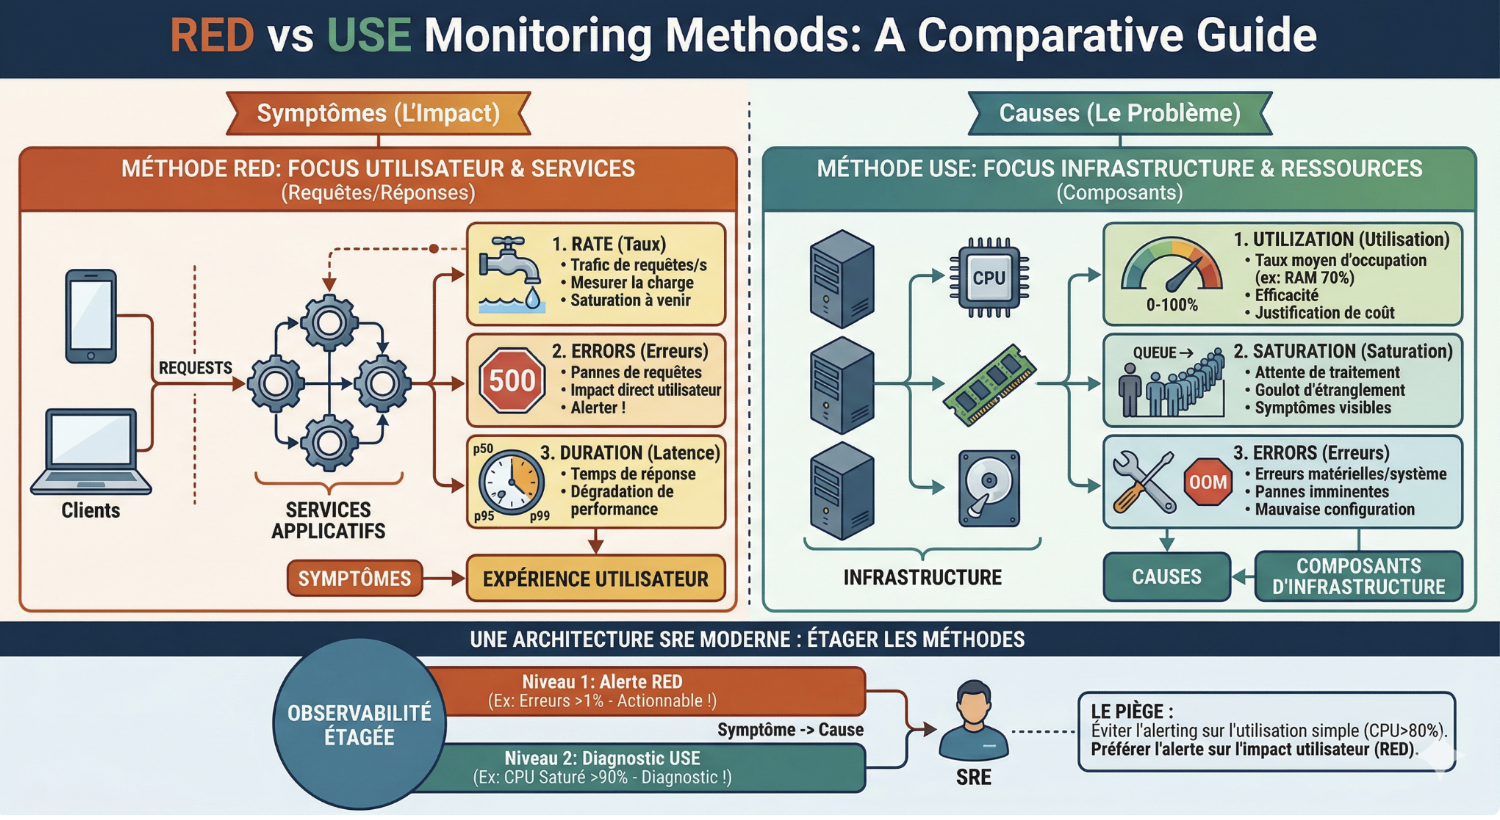
\includegraphics[width=\textwidth]{ressources-graphiques/use_red.png}
	\caption{Comparaison des méthodes RED (côté client) et USE (côté machine)}
	\label{fig:red-use}
\end{figure}
\FloatBarrier

\subsection{La méthode USE (vue côté machine)}

La méthode \lexique{USE} évalue la santé des composants sous-jacents à travers trois dimensions :

\begin{itemize}
	\item \textbf{Utilization} (Utilisation) : le pourcentage de temps pendant lequel une ressource est occupée (par exemple CPU ou RAM à 80 \%).
	\item \textbf{Saturation} : la quantité de travail en attente que la ressource ne peut traiter immédiatement (par exemple la longueur d'une file d'attente).
	\item \textbf{Errors} (Erreurs) : le nombre d'erreurs matérielles ou système survenues (par exemple UnHealthyHostCount).
\end{itemize}

L'objectif de la méthode USE est d'identifier les goulots d'étranglement matériels avant qu'ils ne
fassent tomber le service. Elle répond à la question « pourquoi » du point de vue de la machine.

\subsection{La méthode RED (vue côté client)}

La méthode \lexique{RED} se concentre sur les requêtes applicatives, au plus près de
l'expérience utilisateur, à travers trois dimensions :

\begin{itemize}
	\item \textbf{Rate} (Débit) : le nombre de requêtes par seconde reçues par le service.
	\item \textbf{Errors} (Erreurs) : le nombre de requêtes qui échouent.
	\item \textbf{Duration} (Durée) : le temps nécessaire pour traiter les requêtes, c'est-à-dire la latence.
\end{itemize}

L'objectif de la méthode RED est de mesurer directement la qualité de l'expérience utilisateur et la
santé des microservices. Elle répond à la question « y a-t-il un problème » du point de vue du client.

En résumé, le RED nous dit qu'il y a un problème pour l'utilisateur, tandis que le USE nous aide à
comprendre pourquoi du point de vue de la machine. C'est la combinaison de ces deux vues qui
permet à la fois d'alerter au bon moment et de diagnostiquer rapidement.

\section{Des \lexique{métriques} d'application au cœur de l'alerting}

Le principal levier de la nouvelle solution consiste à déplacer l'alerting des \lexique{métriques} d'infrastructure
vers les \lexique{métriques} d'application. Jusqu'ici, les alertes reposaient presque exclusivement sur des
indicateurs techniques collectés par CloudWatch — par exemple une alarme du type
\texttt{CPUUtilization > 80 \%} pendant cinq minutes. Ces signaux décrivent l'état des machines, mais
pas ce que vivent réellement les joueurs.

Or la plateforme dispose déjà d'une source riche d'informations applicatives. Les services de Winamax
communiquent entre eux via des API au format \lexique{JSON-RPC} : un protocole simple où un service en appelle
un autre en lui envoyant un message structuré en JSON (le format texte standard d'échange de données
sur le web). Toutes ces requêtes traversent un \emph{\lexique{middleware}} — une couche logicielle commune,
placée sur le chemin de chaque appel, qui les traite de façon transparente sans que chaque équipe ait à
la réécrire.

Ce middleware est \emph{instrumenté} avec \lexique{OpenTelemetry}, un standard d'observabilité : à chaque
requête, il produit automatiquement de la télémétrie qui décrit ce qui s'est passé. C'est à partir de cette instrumentation que sont ensuite calculées des \lexique{métriques}
applicatives — nombre de requêtes, taux d'erreur, temps de réponse — qui sont exportées vers AMP
(Amazon Managed Service for \lexique{Prometheus}). Ces \lexique{métriques} existaient donc déjà, mais n'étaient pas
exploitées pour l'alerting. Les brancher à la chaîne d'alerte constitue le cœur de ma contribution : elles
permettent d'alerter au niveau du métier — le comportement des services tel que les joueurs le
perçoivent — et non plus seulement au niveau des ressources techniques.

Cette bascule est rendue possible par \lexique{Prometheus} et son langage de requêtes, PromQL. Il permet
d'exprimer des conditions fines et directement liées à l'expérience utilisateur. Sur cette base, j'ai
standardisé trois \lexique{métriques} appliquées aux API de la plateforme :

\begin{itemize}
	\item \textbf{Latency P99} : mesure du temps de réponse sous laquelle s'exécutent 99 \% de vos requêtes ;
	\item \textbf{Error Rate} : la proportion de requêtes en échec, calculée à partir du statut \lexique{JSON-RPC} renvoyé par chaque service ;
	\item \textbf{Service Down} : la chute anormale du volume de requêtes reçues par un service, signe qu'il ne répond plus.
\end{itemize}

Prises ensemble, ces \lexique{métriques} traduisent directement l'impact sur l'utilisateur : une hausse du taux
d'erreur sur l'API de dépôt signale immédiatement qu'un joueur ne parvient plus à déposer d'argent —
une information bien plus actionnable qu'un simple pic de CPU.

\section{Les niveaux de criticité}

Afin de ne solliciter les équipes d'astreinte qu'en cas de problèmes réellement critique, un niveau de
criticité est attribué à chaque alerte, sous forme de tags ou de labels sur les règles \lexique{Prometheus}. Quatre
niveaux ont été définis.

\begin{table}[h]
	\centering
	\caption{Niveaux de criticité de la nouvelle solution d'alerting}
	\label{tab:niveaux-criticite}
	\begin{tabular}{|p{0.15\textwidth}|p{0.45\textwidth}|p{0.3\textwidth}|}
		\hline
		\textbf{Niveau} & \textbf{Définition} & \textbf{Exemples} \\
		\hline
		P1 -- Critical & Erreur critique ayant un impact direct et important sur l'utilisateur ; doit être résolue le plus rapidement possible. & L'utilisateur ne peut plus déposer d'argent ; plus aucun accès à un service. \\
		\hline
		P2 -- High & Problème important dégradant l'expérience ; le service reste utilisable mais l'astreinte doit être alertée. & Plus de 2 s d'attente avant de jouer au poker ; page de betting chargée en 5 s. \\
		\hline
		P3 -- Warning & Approche de la saturation d'un composant ; pas de réveil de l'astreinte. Une P3 peut devenir P2 si elle dure. & Utilisation CPU > 80 \% ; RAM > 80 \%. \\
		\hline
		P4 -- Info & Information sur l'état du système, à des fins d'observabilité. & Suivi de l'utilisation des CPU, de la RAM, etc. \\
		\hline
	\end{tabular}
\end{table}

Cette hiérarchisation est essentielle : elle établit un langage commun entre les équipes et fonde toute
la logique de routage décrite ci-après. Elle traduit également un changement de culture, en assumant
que toutes les anomalies ne se valent pas et que certaines n'ont pas vocation à interrompre une
astreinte.

\section{Stratégie de notification et matrice de routage}

Le choix du canal de notification dépend à la fois de la priorité de l'alerte et de l'environnement
concerné. L'objectif est de réveiller une personne uniquement lorsque cela est justifié, et de router
les autres alertes vers des canaux consultables sans urgence.

\begin{table}[h]
	\centering
	\caption{Matrice de routage des alertes selon la priorité et l'environnement}
	\label{tab:matrice-routage}
	\begin{tabular}{|p{0.2\textwidth}|p{0.25\textwidth}|p{0.45\textwidth}|}
		\hline
		\textbf{Priorité} & \textbf{Environnement} & \textbf{Canal principal} \\
		\hline
		P1 -- Critical & PROD & SMS + Slack (\texttt{\#alerts-\$\{TEAM\}-\$\{ENV\}}) \\
		\hline
		P2 -- High & PROD & SMS + Slack (\texttt{\#alerts-\$\{TEAM\}-\$\{ENV\}}) \\
		\hline
		P3 -- Warning & PROD & Slack (\texttt{\#alerts-\$\{TEAM\}-\$\{ENV\}}) \\
		\hline
		Toutes & DEV / PRELIVE & Slack (\texttt{\#\$\{TEAM\}-\$\{ENV\}}) \\
		\hline
		\lexique{Logs} & Tous & Slack (\texttt{\#\$\{TEAM\}-logs-\$\{ENV\}}) \\
		\hline
	\end{tabular}
\end{table}

En dehors de la production, même une alerte P1 ne doit pas déranger l'astreinte : un simple message est envoyé sur le canal Slack dédié à l'équipe
concernée. En revanche, pour les alertes P1 et P2 en production, il est impératif de réveiller la personne
d'astreinte, en plus de l'envoi du message sur le canal de l'équipe impactée. Chaque équipe dispose ainsi de ses propres canaux, ce qui garantit
que l'alerte parvient bien à la personne experte du service en cause.

\section{Corrélation RED / USE et runbooks}

Afin d'améliorer le temps moyen de réparation (MTTR), les alertes \lexique{RED} de criticité « Critical » ou
« High » sont associées aux alertes \lexique{USE} « Warning » du même service. Cette corrélation facilite le diagnostic pour la personne d'astreinte : plutôt que de recevoir
une alerte isolée, elle dispose immédiatement des pistes de cause possibles. Par exemple, si le service
\texttt{betting-api} signale un dépassement du seuil de latence P99 pendant plus de cinq minutes,
l'alerte intègre les warnings susceptibles d'en être la cause, comme un ralentissement dans la lecture
d'une base de données.

En plus de cela, chaque alerte doit être associée à un runbook — une fiche décrivant la marche à suivre pour
diagnostiquer et résoudre le problème — et à un lien direct vers un \lexique{dashboard}
Grafana du service concerné. Ce \lexique{dashboard} offre une visualisation détaillée permettant d'identifier
rapidement la ou les fonctions problématiques du service. Le runbook constitue ainsi un point d'entrée
unique pour comprendre l'alerte et engager la résolution, sans perte de temps en recherche
d'informations.

